\documentclass[11pt,titlepage]{article}
\usepackage{fullpage}
\usepackage{amsmath}
\usepackage{amssymb}
\usepackage{gensymb}
\usepackage{color}
\usepackage{bm}
\usepackage{graphicx}
\graphicspath{ {images/} }
\usepackage{tikz}
\usetikzlibrary{shapes,arrows,positioning,calc}
\usepackage{float}
\restylefloat{table}
\usepackage{array}
\tikzset{
    block/.style = {draw, fill=white, rectangle, minimum height=3em, minimum width=3em},
    sum/.style = {draw, fill=white, circle, node distance=1cm},
    input/.style = {draw=none},
    output/.style = {draw=none},
    coord/.style = {coordinate}
}

\author{Rane Brown \\ Kate Schneider}
\title{ECEN 4638: Lab W}
\date{\today}

\begin{document}
\maketitle
\tableofcontents
\listoffigures
\newpage

\section{Description}
The goal of this lab is to investigate the response of a two disc system when proportional control is used. System parameters are determined through experimental data collection and analysis, and the response of the physical system is compared to the expected response based on an LTI model.

\section{Setup}
In this experiment, we set up the Torsion Disc System to use two discs. The bottom disc is configured with 4 weights mounted at \textcolor{red}{6cm??} from the center rod, and the top disc is configured in multiple configurations for manual system excitation and data collection: \\\\
1.) 2 weights mounted at 6cm\\
2.) 2 weights mounted at 9cm\\
3.) 4 weights mounted at 6cm.\\\\
The final configuration was also used for frequency analysis with the motor control on.

\section{System model}
	\subsection{LTI model}	
	With a two disc system, our model becomes more complex, as we must now take into consideration the position and velocity of each disk. The additional dynamics introduce the quantities $k$, the spring constant, and $c_2$, the damping ratio of the second disc. The two disc system can be modeled as:
	\begin{align}
		J_1\ddot \theta_1+c_1\dot \theta_1+k(\theta_1-\theta_2)=bu \\
		J_2\ddot \theta_2+c_2\dot \theta_2+k(\theta_2-\theta_1)=0
	\end{align}
	
	 The difference in position of the discs, $\beta$ is also of interest, where $\beta = \theta_1-\theta_2$. If we make this substitution, as well as substituting in angular velocity $\omega$ for $\dot \theta$, our system becomes:
	 \begin{align}
	 	J_1\dot \omega_1+c_1\omega_1+k\beta=bu \\
		J_2\dot \omega_2+c_2\omega_2-k\beta=0
	 \end{align}
	 
	 \subsection{Transfer functions}
	 For this experiment, there are three transfer functions of interest: the transfer function from the motor voltage control $u\mapsto\omega_1$, $u\mapsto\omega_2$, $u\mapsto\beta$. These can be determined by solving the system in the Laplace domain, or by using a state-space model of the system
	 
	 \[
	\begin{bmatrix}
		\dot \omega_1\\
		\dot \omega_2\\
		\dot \beta
	\end{bmatrix}=
  	\begin{bmatrix}
    		-\frac{c_1}{J_1} & 0 & -\frac{k}{J_1} \\
	    	0 & -\frac{c_2}{J_2} & -\frac{k}{J_2}\\
		1 & -1 & 0
  	\end{bmatrix}
	\begin{bmatrix}
		\omega_1\\
		\omega_2\\
		\beta
	\end{bmatrix}+
	\begin{bmatrix}
		\frac{b}{J_1}\\
		0\\
		0
	\end{bmatrix}
	\]
	
	and solving for the transfer functions with 
	\begin{align}
		\hat{x}(s) = (sI-A)^{-1}=b\hat{u}(s).
	\end{align}
	 Using the latter method, we obtain the transfer functions of interest:\\
	 \begin{align}
	  	H_{\omega_{1}u}(s)= \frac{\frac{b}{J_1}(s^2+\frac{c_2}{J_2}s+\frac{k}{J_2})}{s^3+(\frac{c_1}{J_1}+\frac{c_2}{J_2})s^2+(\frac{c_1}{J_1}\frac{c_2}{J_2}+\frac{k}{J_2}+\frac{k}{J_2})s+(\frac{k}{J_1}\frac{c_2}{J_2}+\frac{k}{J_2}\frac{c_1}{J_1})} \\
	  	H_{\omega_{2}u}(s)= \frac{\frac{b}{J_1}\frac{k}{J_2}}{s^3+(\frac{c_1}{J_1}+\frac{c_2}{J_2})s^2+(\frac{c_1}{J_1}\frac{c_2}{J_2}+\frac{k}{J_2}+\frac{k}{J_2})s+(\frac{k}{J_1}\frac{c_2}{J_2}+\frac{k}{J_2}\frac{c_1}{J_1})}\\
	  	H_{\beta u}(s)=\frac{\frac{b}{J_1}(s+\frac{c_2}{J_2})}{s^3+(\frac{c_1}{J_1}+\frac{c_2}{J_2})s^2+(\frac{c_1}{J_1}\frac{c_2}{J_2}+\frac{k}{J_2}+\frac{k}{J_2})s+(\frac{k}{J_1}\frac{c_2}{J_2}+\frac{k}{J_2}\frac{c_1}{J_1})}
	  \end{align}\\
	  
	  It should be noted that these transfer functions have the same poles and different zeros, as is expected. In this lab, we are interested in a collocated system in which sensing and actuation occur at the same place. For this reason, $\omega_1$ is fed back into our system, and the transfer function of greatest interest to us is $H_{\omega_{1}u}(s)$.

\section{Manual determination of system parameters}
	System parameters spring constant $k$ and damping ratio $c_2$ can be determined by manual oscillation of the system and Matlab analysis of the results. To determine these parameters, we manually oscillate the bottom disc and record the position of both the top and bottom disc. The position information of each disc is recorded in LabView, and is imported into Matlab for processing using the \texttt{accel\_fir.m} and \texttt{conv\_delay.m} scripts to obtain filtered position data. We can then use a least-squares approach to determine $c_2$ and $k$ for each configuration of weights that was tested. The least-squares evaluation is set up as:
	\begin{align}
	\begin{bmatrix}
		\dot \theta_2 & \theta_1-\theta_2
	\end{bmatrix} 
	\begin{bmatrix}
		c\\
		k
	\end{bmatrix}&=
	\begin{bmatrix}
		-J_2\ddot \theta_2
	\end{bmatrix}\\
	\bm{A}x&=\bm{B}
	\end{align}
	
	Where $c_2$ and $k$ can be found by $x=\bm{A}$\textbackslash$\bm{B}$. The results for the various weight configurations of disc 2 are:\\\\
	
	        \begin{table}[H]
            \centering
            \begin{tabular}{|m{4cm}|m{3cm}|m{3cm}|m{3cm}|} 
                \hline
                Weight distribution disc 2 & $J_2$ & $c_2$ & $k$ \\ 
                \hline
                2 weights at 6cm & 0.0058 & 0.0093 & 2.059\\
                \hline
                2 weights at 9cm & 0.0103 & 0.018 & 2.1231\\
                \hline
                4 weights at 6cm & 0.0097 & 0.0107 & 2.2306\\
                \hline
            \end{tabular}
            \caption{Data Collection Parameters} \label{table:data_param}
        \end{table}

	Taking the average, we obtain $c_2 = 0.0107$ and $k=2.1822$.
	
	
\section{System stability}
	\subsection{Root locus analysis}
	From the transfer functions for our system as well as the manually determined system parameters, we can estimate our system's stability before the introduction of a controller. This is accomplished by plotting the root locus of the system to determine whether, and at what gain, the system becomes unstable. The root locus plot for the transfer function $H_{\omega_{1}u}(s)$ with 2 weights at 6cm for the top disc is shown below. 
	\begin{figure}[H]
            \centering
            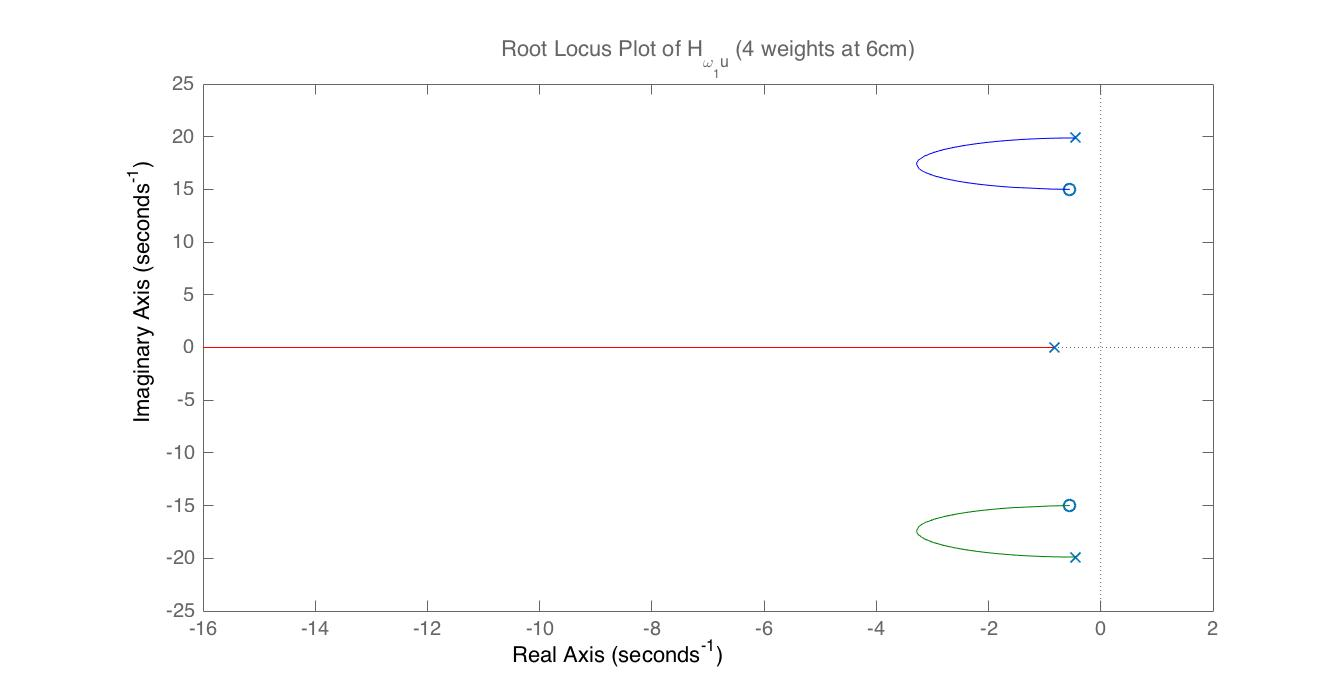
\includegraphics[trim={6cm 0 1cm 1cm},clip,origin=c,scale=0.26]{rlplot_4w_6cm_2disks}
            \caption{Root Locus Plot $H_{\omega_{1}u}$}
            \label{fig:disc_sys}
       \end{figure}
       
       From the root locus plot, it can be seen that the system, theoretically, should not go unstable no matter how large the gain is. However, we know from previous experiments that this is not the case. Our system has additional dynamics at play which are not accounted for in our model. The roots of our system occur at $s=-0.4456 \pm 19.9j$ and $s=-0.827$. 
       
       We can also look at the root locus plots of the transfer functions $H_{\omega_{2}u}(s)$ and $H_{\beta u}(s)$, to see how the different zeros affect stability. These plots are included below.
       \begin{figure}[H]
            \centering
            \begin{minipage}{.5\textwidth}
                \centering
              	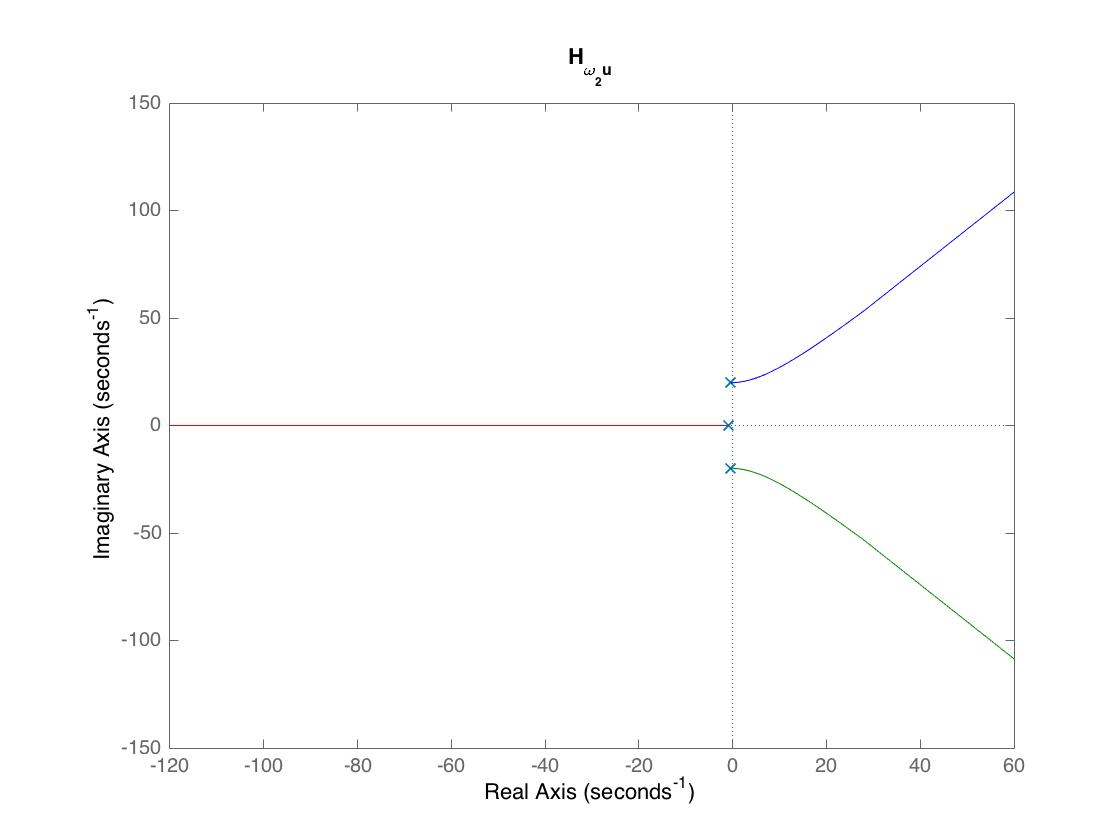
\includegraphics[trim={6cm 0 0 0},clip,origin=c,scale=0.25]{rlplot_w2}
            	\caption{Root Locus Plot $H_{\omega_{2}u}$}
           	\label{fig:disc_sys}
            \end{minipage}%
            \begin{minipage}{.5\textwidth}
                \centering
                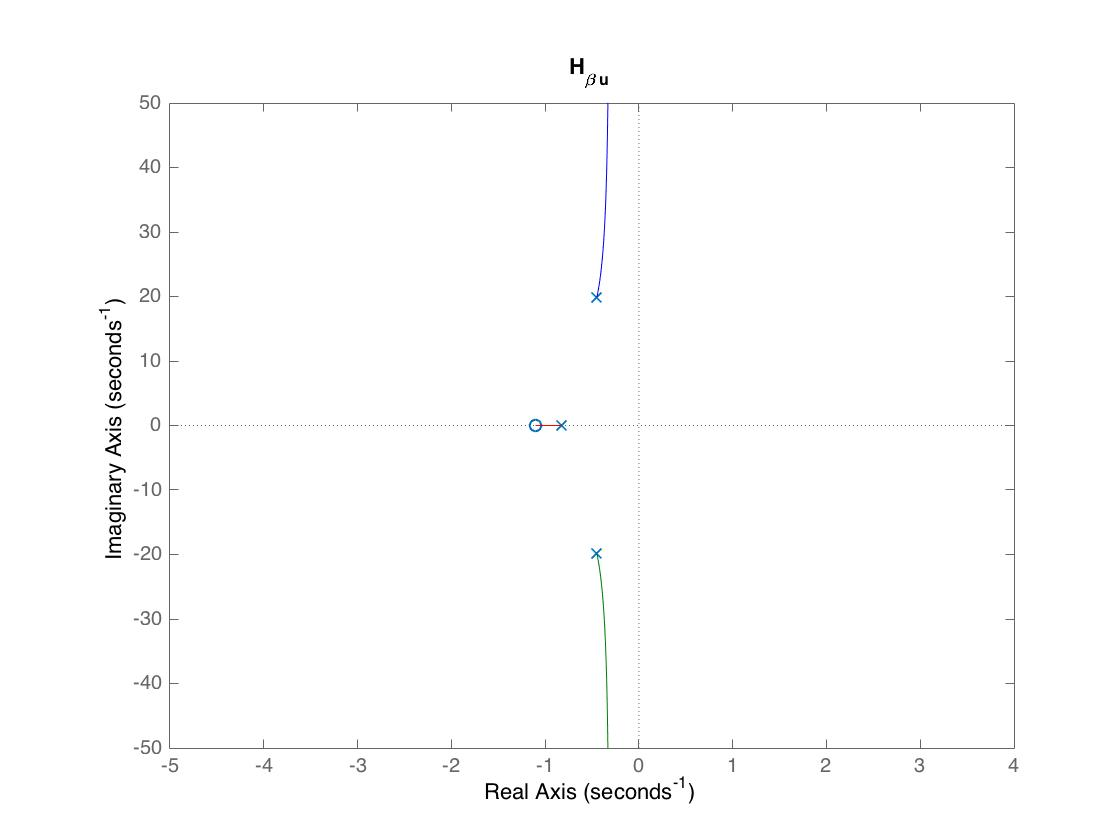
\includegraphics[trim={6cm 0 0 0},clip,origin=c,scale=0.25]{rlplot_B}
            \caption{Root Locus Plot $H_{\beta u}$}
            \label{fig:disc_sys}
            \end{minipage}%
       \end{figure}
       
	
	\subsection{Routh's stability criterion}
	Another way to determine system stability is via Routh's stability criterion. This can also be calculated for our system using our manually determined parameters $c_1$, $c_2$, and $k$:\\\\
	$\begin{matrix}
		s^3: & 1 & 396.182\\
		s^2: & 1.72 & 327.05\\
		s^1: & 206.0367 & 0\\
		s^0: & 327.05 & 0
	\end{matrix}$\\

Since there are no sign changes in the first column of our Routh array, we can confirm that the theoretical system should be stable.

	\subsection{Theoretical Bode analysis}
	With our system parameters, we can also plot the frequency response of the transfer functions of interest. These plots are included below for comparison to the frequency response determined experimentally, which is discussed further in \textcolor{red}{section ?}. 
	
	\begin{figure}[H]
            \centering
            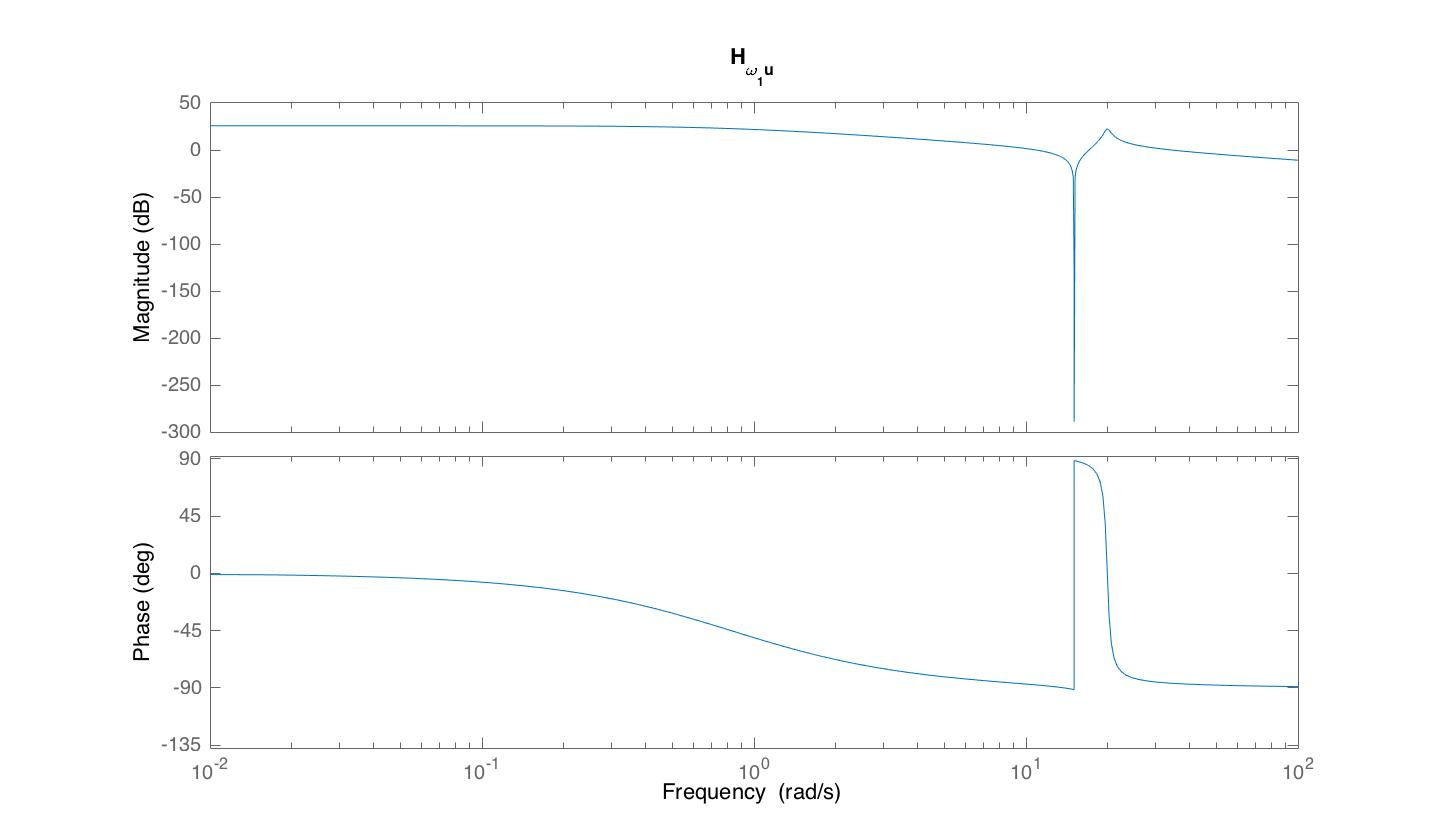
\includegraphics[trim={6cm 0 1cm 1cm},clip,origin=c,scale=0.26]{w1_bode}
            \caption{Frequency Response $H_{\omega_{1}u}$}
            \label{fig:disc_sys}
       \end{figure}
       
       \begin{figure}[H]
            \centering
            \begin{minipage}{.5\textwidth}
                \centering
              	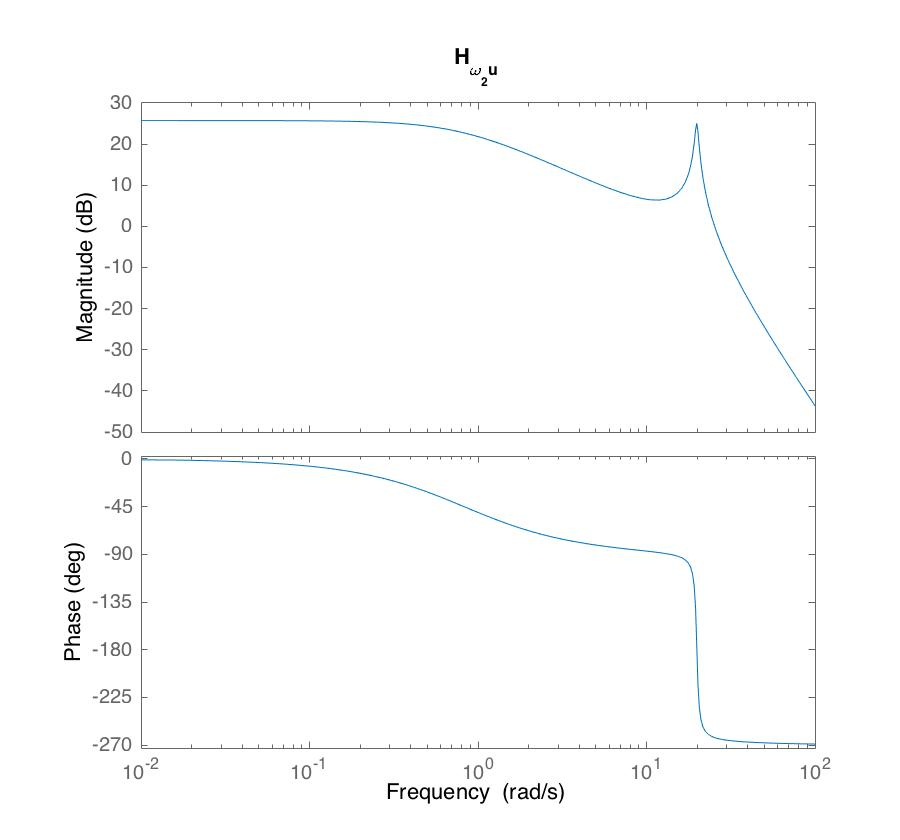
\includegraphics[trim={2cm 0 0 0},clip,origin=c,scale=0.25]{w2_bode}
            	\caption{Frequency Response $H_{\omega_{2}u}$}
           	\label{fig:disc_sys}
            \end{minipage}%
            \begin{minipage}{.5\textwidth}
                \centering
                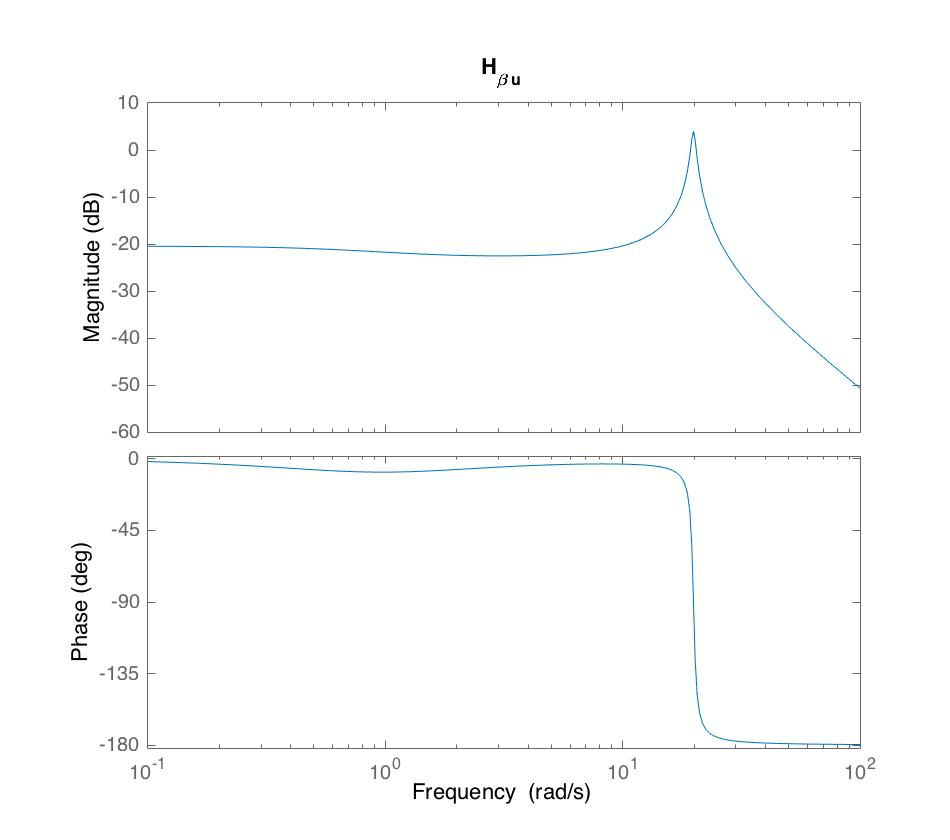
\includegraphics[trim={2cm 0 0 0},clip,origin=c,scale=0.25]{B_bode}
            \caption{Frequency Response $H_{\beta u}$}
            \label{fig:disc_sys}
            \end{minipage}%
       \end{figure}
	
\section{}



\end{document}